\chapter{A search for new phenomena}
\label{chapter:2ljets}

\begin{epigraphs}
\qitem{%
An experiment is never a failure solely because it fails to
achieve predicted results. An experiment is a failure only when it also
fails adequately to test the hypothesis in question, when the data it
produces don’t prove anything one way or another.%
}%
{Robert M. Pirsig~\cite{pirsig1999zen}}
\qitem{%
But there is one feature I notice that is generally missing in cargo cult
science. \ldots\
% That is the idea that we all hope you have learned in studying science in
% school--we never say explicitly what this is, but just hope that you catch
% on by all the examples of scientific investigation. It is interesting,
% therefore, to bring it out now and speak of it explicitly.
It's a kind of scientific integrity, a principle of scientific thought that
corresponds to a kind of utter honesty --- a kind of leaning over backwards.%
}%
{Richard Feynman~\cite{feynman1974cargo}}
\end{epigraphs}


Our central result is Figure~\ref{fig:2ljets_summary}, which shows the names,
data, and fitted background expectations with error bars in all main regions.
This figure illustrates the background-model part of a \clown{likelihood}
function which is extended with signals to test alternative models.
Exclusion contours testing the addition of C1N2 and GMSB signals to these
backgrounds are shown in Figure~\ref{fig:2ljets_contours}.


\begin{figure}[tp]
\centering
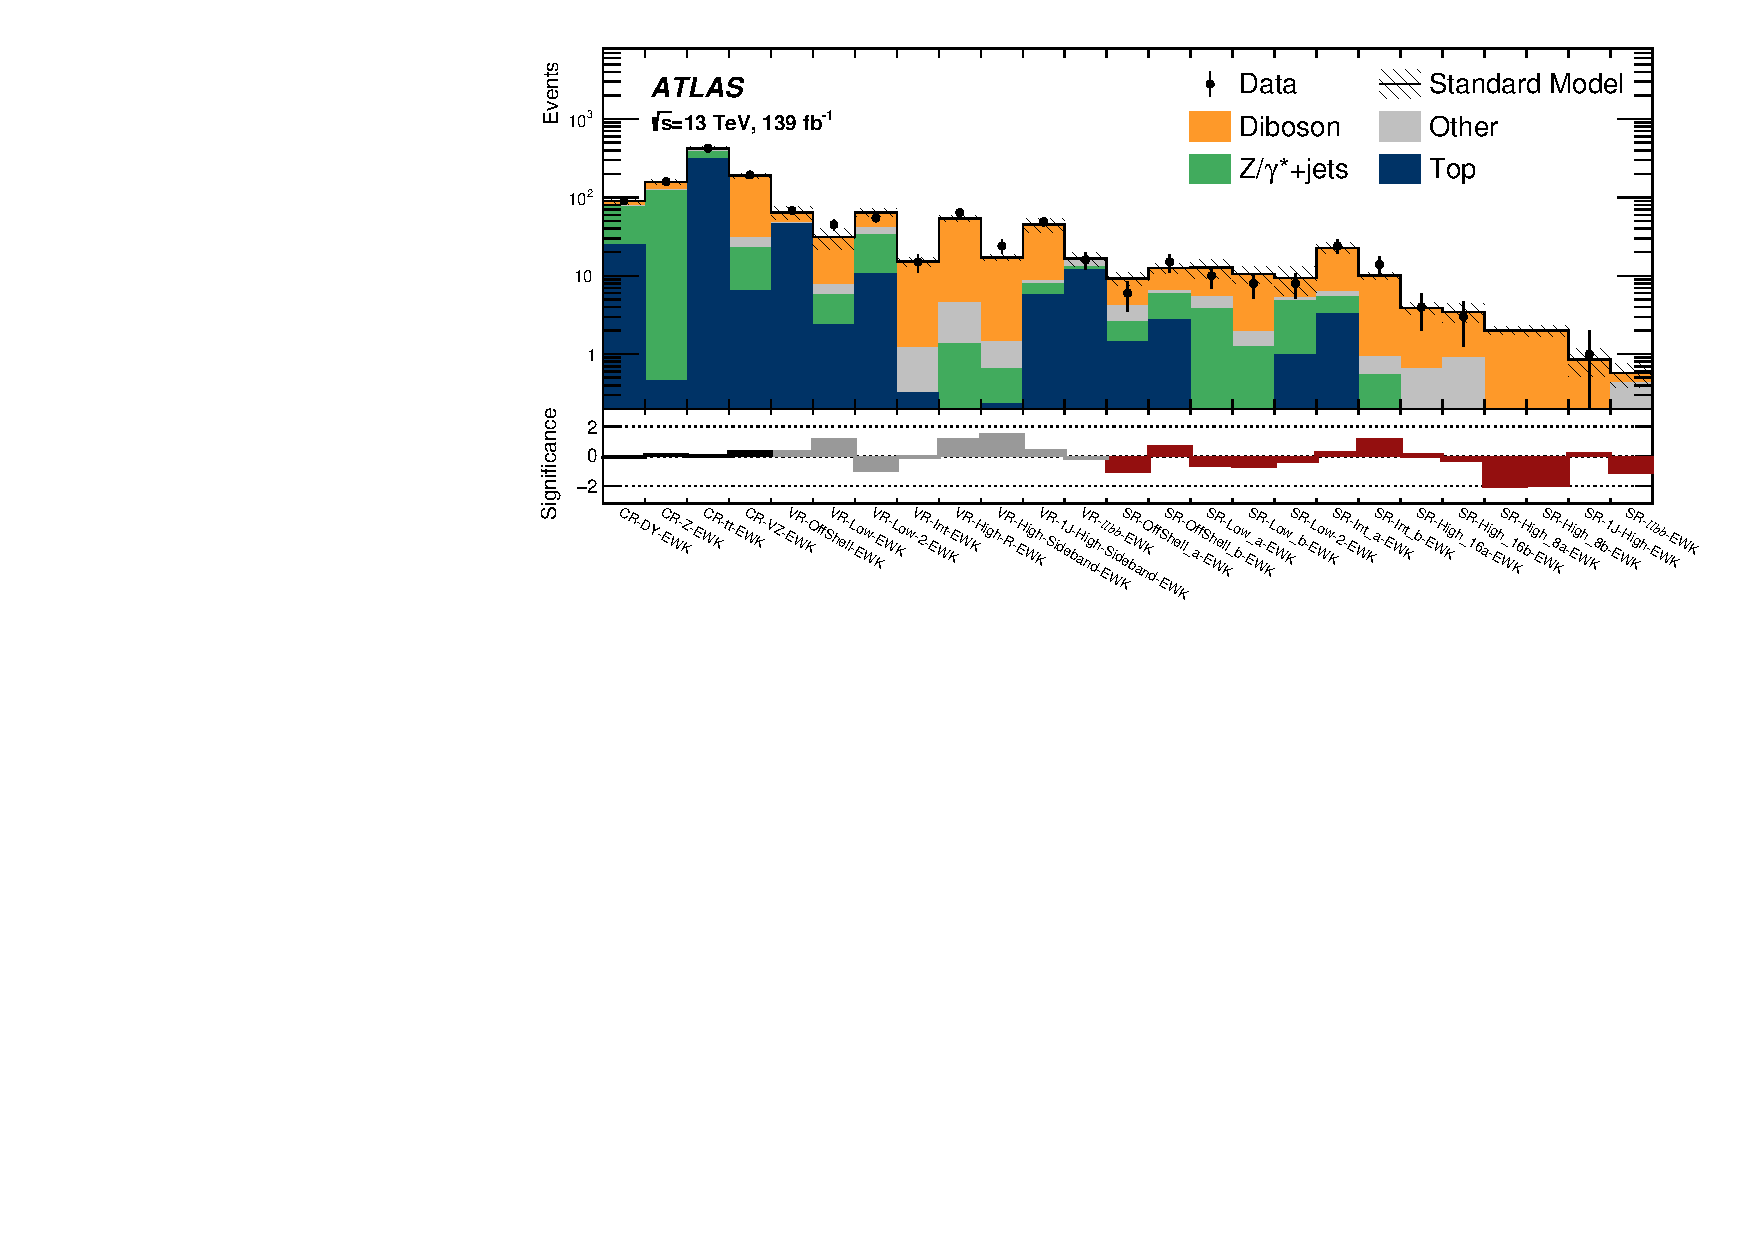
\includegraphics[width=\textwidth]{figures/2ljets_summary_log.pdf}
\caption{%
Data of the $\twoljets$ electroweak analysis with \emph{post-fit} backgrounds
for which the lower panel shows $S_\mathrm{ATLAS}$ from
Equation~\ref{eqn:significance_atlas}.
Control, validation and signal regions are shown from left to right, with the
regions within each category ordered approximately by their typical $\ptmiss$.
Likelihoods from validation regions are not included in the fit.
The `Top' category contains $t\bar t$ and $tW$ processes, and
`Other' contains fake/non-prompt lepton, higgs, triboson, $t\bar tZ$, and other
rare top processes.%
}
\label{fig:2ljets_summary}
\end{figure}


\begin{figure}[tp]
\centering
\begin{subfigure}{\textwidth}
    \centering
    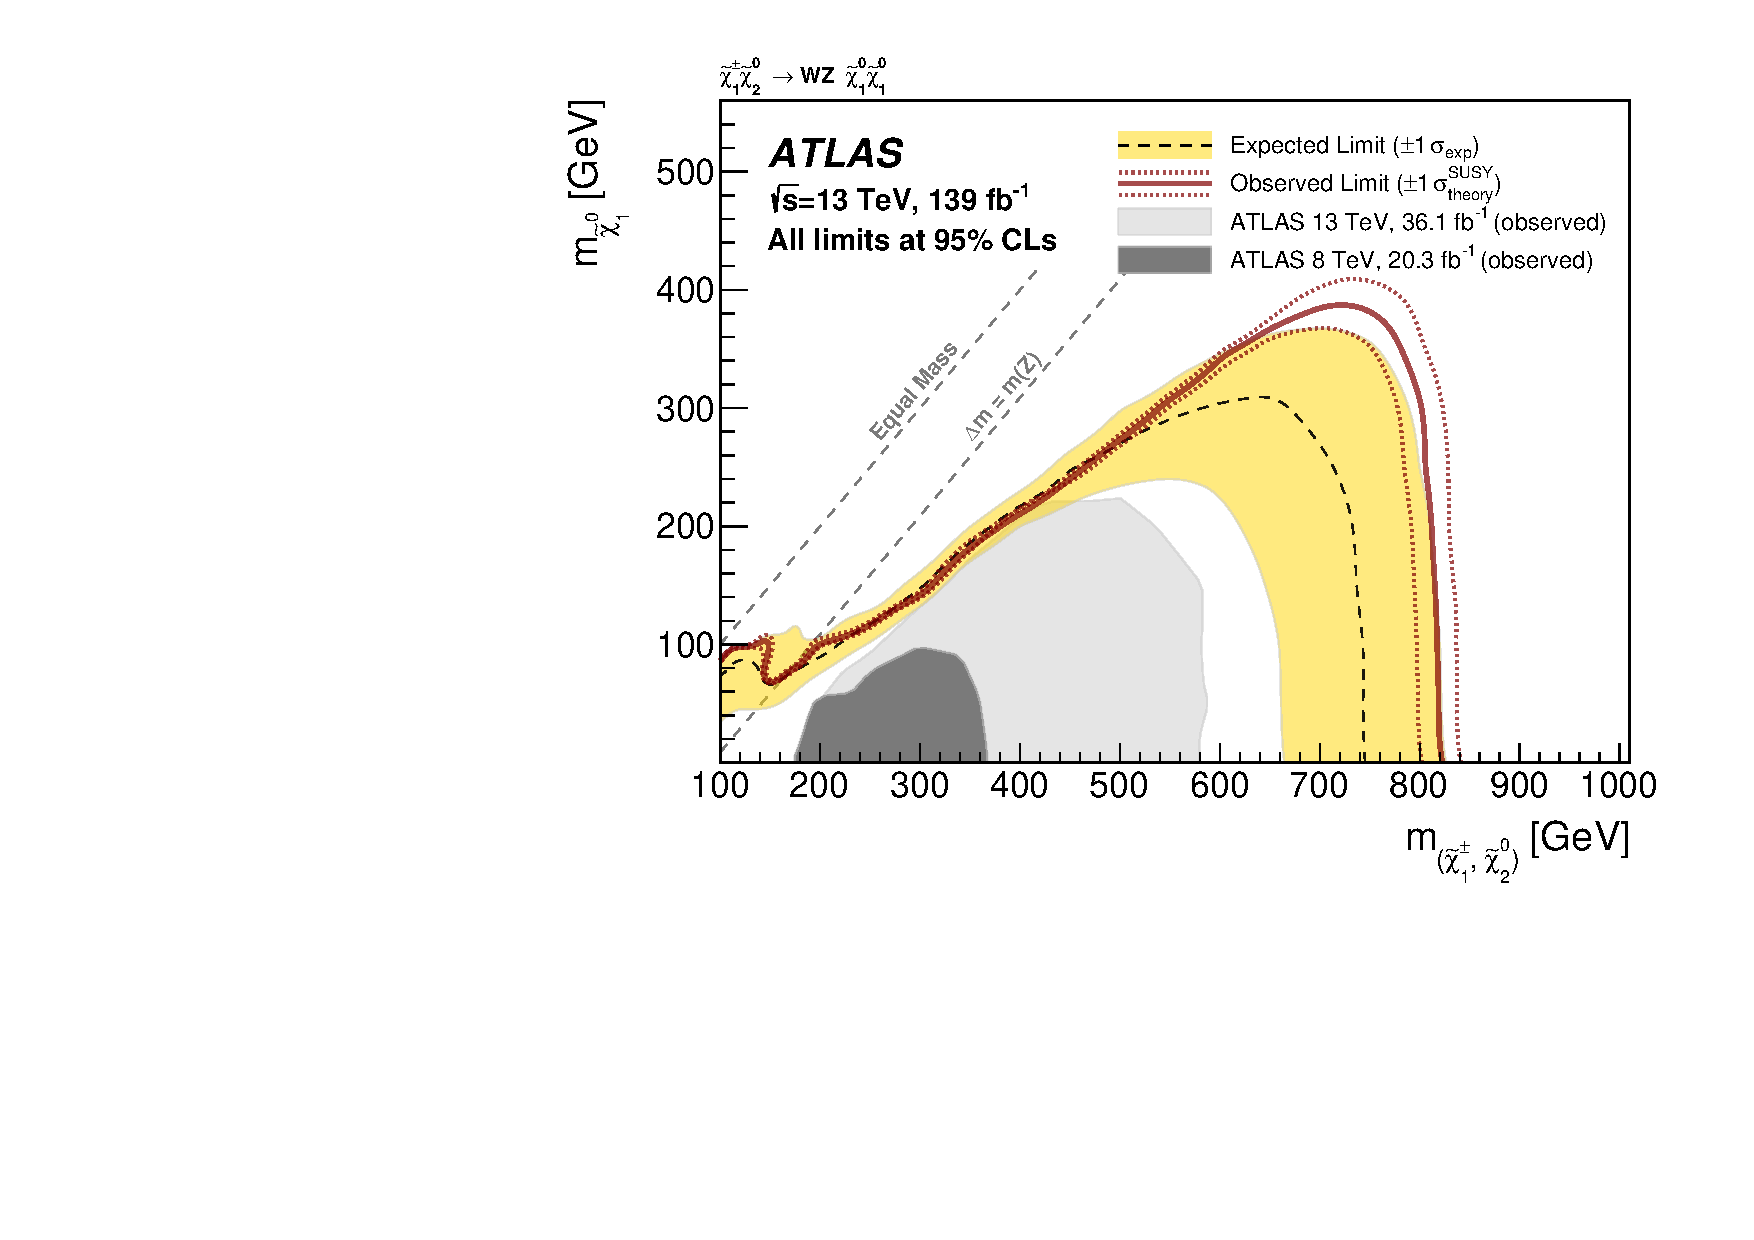
\includegraphics[width=0.7\textwidth]{figures/2ljets_contours_c1n2.pdf}
    \caption{C1N2 contours}
\end{subfigure}
\\[1em]
\begin{subfigure}{\textwidth}
    \centering
    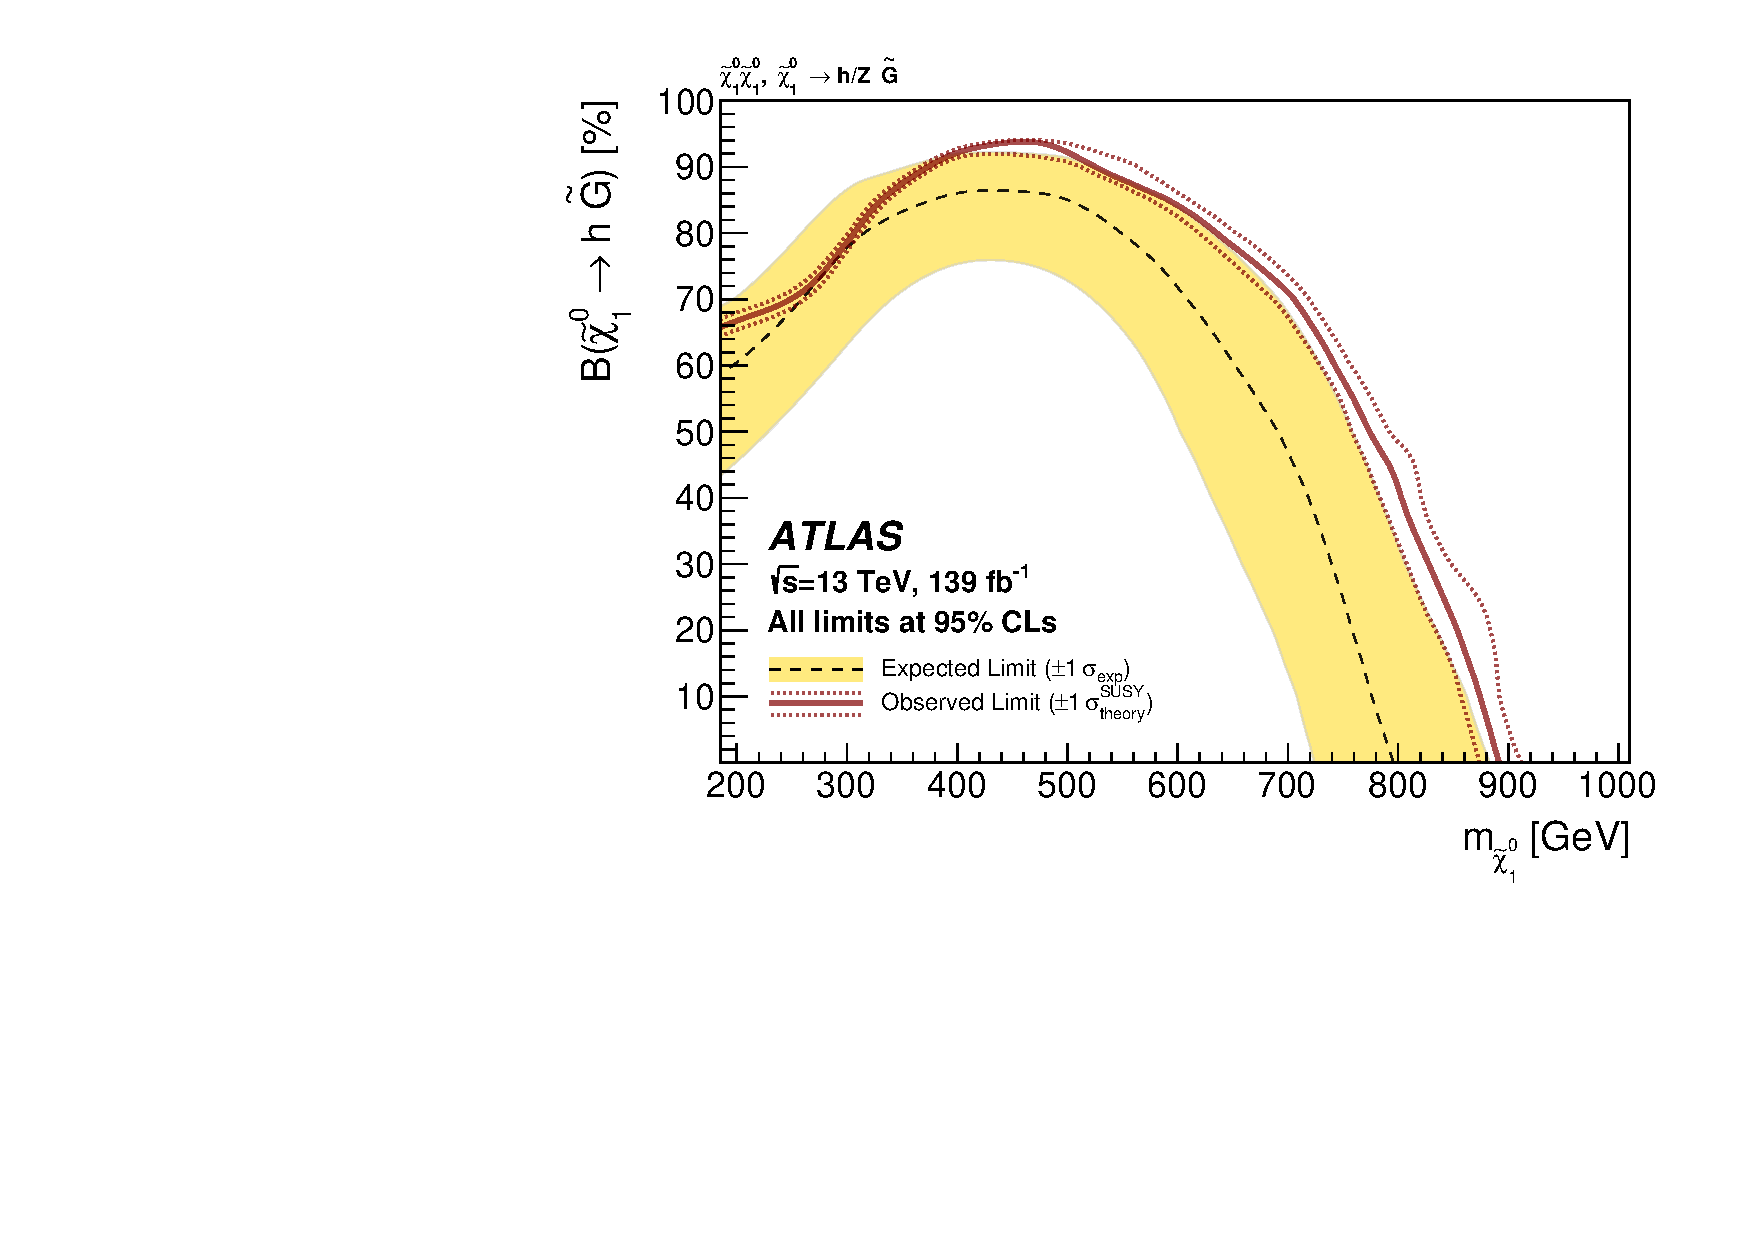
\includegraphics[width=0.7\textwidth]{figures/2ljets_contours_gmsb.pdf}
    \caption{GMSB contours}
\end{subfigure}
\caption{%
Contours from the $\twoljets$ electroweak analysis for
C1N2 (top) and GMSB (bottom) models.
Space below the solid red line is labelled as excluded and its dotted
neighbours show the result if all signal cross-sections are varied up and down
by theoretical error bars.
The yellow band shows the prior $\pm1$-sigma region of exclusion contours
from asymptotic approximations to the distribution of the test statistic.
Grey areas are observed limits from the $2\ell$ parts
of~\cite{SUSY-2016-24} and~\cite{SUSY-2013-11}.
Exclusion is defined by the $\mathrm{CLs}$ prescription at the $0.05$ level
in asymptotic approximations.
All contours are interpolated from a sparse grid.
}
\label{fig:2ljets_contours}
\end{figure}
